
%(BEGIN_QUESTION)
% Copyright 2007, Tony R. Kuphaldt, released under the Creative Commons Attribution License (v 1.0)
% This means you may do almost anything with this work of mine, so long as you give me proper credit

Noen strømningsmåleinstrumenter er av {\it innstikk}-typen, som dette Annubar-instrumentet.  Her går Annubar-røret gjennom midten av en kuleventil, med en kompresjonsferrule og mutter som tetter så prosessvæsken ikke lekker ut av monteringen:

$$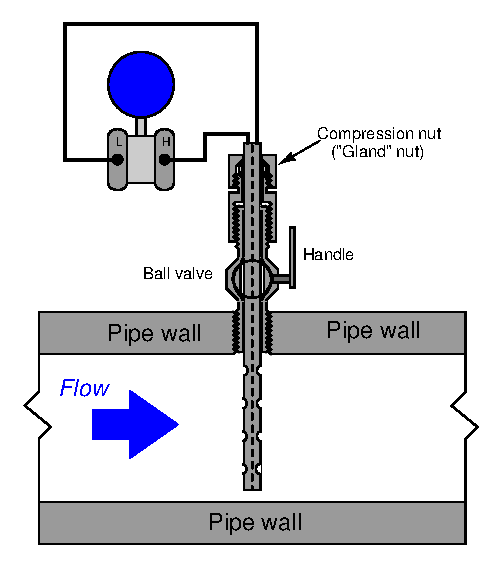
\includegraphics[width=15.5cm]{i00047x01.eps}$$

Beskriv hvordan et innstikk-flowmeter som dette kan fjernes fra et rør i drift, og deretter installeres igjen, {\it uten å avbryte strømmen av prosessvæske gjennom røret}.


\underbar{file i00047}
%(END_QUESTION)





%(BEGIN_ANSWER)

For å fjerne:

\begin{itemize}
\item{} Løsne pakkboks-/glandmutteren til innstikkhuset kan bevege seg opp og ned
\item{} Trekk Annubar-enheten ut av røret til enden klarerer kuleventilen
\item{} Steng kuleventilen
\item{} Skru av pakkboks-/glandmutteren helt
\item{} Trekk Annubar helt ut av røret
\end{itemize}

\vskip 10pt

For å installere på nytt, reverser alle trinn!

%(END_ANSWER)





%(BEGIN_NOTES)


%INDEX% Measurement, flow: servicing an insertion-type flowmeter

%(END_NOTES)
